\documentclass{standalone}
\usepackage{pgfplots, tikz}
\usetikzlibrary{calc, arrows.meta}
\usepackage{colortbl}
\def\mutcell{\cellcolor{lightgray}\color{black}}
\begin{document}
	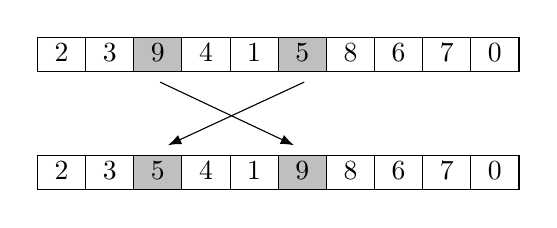
\begin{tikzpicture}
	\node[anchor=center] (start) at (0, 0) {%
		\begin{tabular}{|*{10}{c|}} \hline 
			2 & 3 & \mutcell 9 &  4 &  1 & \mutcell 5 & 8 & 6 & 7 & 0 \\ \hline 
		\end{tabular}};
	\node[anchor=center] (end) at (0, -1.5) {%
		\begin{tabular}{|*{10}{c|}} \hline 
			2 & 3 & \mutcell 5 &  4 &  1 & \mutcell 9 & 8 & 6 & 7 & 0 \\ \hline 
		\end{tabular}};
	\draw[-Latex] ($(start.south) + (0.33, 0)$) -- ($(end.north) + (-1.4,0)$);
	\draw[-Latex] ($(start.south) + (-1.5, 0)$) -- ($(end.north) + (0.2,0)$);
%	\draw[->] ($(start.south) + (-1.5, 0)$) -- ($(end.north) + (-0.95,0)$);
%	\draw[->] ($(start.south) + (-0.4, 0)$) -- ($(end.north) + (-1.4,0)$);
	\end{tikzpicture}
\end{document}